%%%%%%%%%%%%%%%%%%%- HXN
\def\sode{10}

\begin{name}
	{\tenchude}
	{\tendethi}
	{\tentruong}
	{\thoigian}
\end{name}

\caulc
\Opensolutionfile{ans}[ans/ans-HXN-\sode-T]
\begin{ex}%Câu 1
    Trong không gian $Oxyz$, phương trình đường thẳng đi qua điểm $ M\left(1;-3;5\right)$ và có vectơ chỉ phương $\vec{u}=\left(2;-1;1\right)$ là
    \choice
    {$\dfrac{x-1}{2}=\dfrac{y-3}{-1}=\dfrac{z-5}{1}$}
    {$\dfrac{x-1}{2}=\dfrac{y-3}{-1}=\dfrac{z+5}{1}$}
    {\True $\dfrac{x-1}{2}=\dfrac{y+3}{-1}=\dfrac{z-5}{1}$}
    {$\dfrac{x+1}{2}=\dfrac{y+3}{-1}=\dfrac{z-5}{1}$}
\end{ex}

\begin{ex}%Câu 2
\immini
{
        Cho hàm số $ y=\dfrac{ax+b}{cx+d}$ $\left(c\ne 0,ad-bc\ne 0\right)$ có đồ thị như hình vẽ bên. Tiệm cận ngang của đồ thị hàm số là
    \choice
    {$x=-1$}
    {\True $y=\dfrac{1}{2}$}
    {$y=-1$}
    {$x=\dfrac{1}{2}$}
}
{
    \begin{tikzpicture}[line join=round, line cap=round,>=stealth,thick,x=.8cm]
        \tikzset{every node/.style={scale=0.9}}
        \draw[->] (-3,0)--(3,0) node[below left] {$x$};
        \draw[->] (0,-3)--(0,3) node[below left] {$y$};
        \draw (0,0) node [below left] {$O$}
        (0,-0.25)node[below right]{$-\tfrac{1}{4}$}
        (0,0.5)node[above right]{$\frac{1}{2}$};
        \foreach \x/\nx in {-1/-1,1/1}
        \draw[thin] (\x,1pt)--(\x,-1pt) node [below] {$\nx$};
        \draw[dashed,thin] (-0.99,-3)--(-0.99,3);
        \begin{scope}
            \clip (-3,-3) rectangle (3,3);
            \draw[samples=200,domain=-4:-1.01,smooth,variable=\x] plot (\x,{(-1*(\x)+0.5)/(-2*(\x)-2)});
            \draw[samples=200,domain=-0.99:4,smooth,variable=\x] plot (\x,{(-1*(\x)+0.5)/(-2*(\x)-2)});
            \draw[dashed,thin] (-4,1/2)--(4,1/2);
        \end{scope}
    \end{tikzpicture}
}
\end{ex}

\begin{ex}%Câu 3
    Tập nghiệm của phương trình $\log_3\left(18-x^2\right)=2$ là
    \choice
    {$S=\left\{ 3\right\}$}
    {$S=\left\{-3\right\}$}
    {\True $S=\left\{\pm 3\right\}$}
    {$S=\left\{-4;3\right\}$}
\end{ex}

\begin{ex}%Câu 4
    Trong không gian $Oxyz$, mặt phẳng $(P)$ đi qua điểm $ M\left(1;2;3\right)$ và song song với $(Q)\colon x-2y+3z+1=0$ có phương trình là
    \choice
    {$x-2y+3z+6=0$}
    {$x-2y+3z+16=0$}
    {\True $x-2y+3z-6=0$}
    {$x-2y+3z-16=0$}
\end{ex}

\begin{ex}%Câu 5
    Nếu $\int\limits_1^2f(x)\mathrm{\,d}x=-2$ và $\int\limits_2^3f(x)\mathrm{\,d}x=1$ thì $\int\limits_1^3f(x)\mathrm{\,d}x$ bằng
    \choice
    {$-3$}
    {\True $-1$}
    {$1$}
    {$3$}
\end{ex}

\begin{ex}%Câu 6
    Thống kê điểm kiểm tra giữa kỳ 1 môn Toán của $30$ học sinh lớp 12C1 của một trường THPT được ghi lại ở bảng sau:\\
    \centerline{\begin{tblr}{|c|c|c|c|c|}
            \hline
            Điểm & $\left[2;4\right)$ & $\left[4;6\right)$ & $\left[6;8\right)$ & $\left[8;10\right)$\\
            \hline
            Số học sinh & $ 4$ & $ 8$ & $ 11$ & $ 7$\\
            \hline
    \end{tblr}}\\
    Trung vị của mẫu số liệu gốc thuộc khoảng nào trong các khoảng dưới đây?
    \choice
    {$\left[2;4\right)$}
    {$\left[4;6\right)$}
    {\True $\left[6;8\right)$}
    {$\left[8;10\right)$}
\end{ex}

\begin{ex}%Câu 7
    Cho cấp số cộng $\left(u_n\right)$ với $u_{10}=25$ và công sai $d=3$. Khi đó $u_1$ bằng
    \choice
    {$u_1=2$}
    {$u_1=3$}
    {$u_1=-3$}
    {\True $u_1=-2$}
\end{ex}

\begin{ex}%Câu 8
    Cho hình chóp $S.ABC$ có đáy $ABC$ là tam giác vuông tại $B$ và $SA\perp\left(ABC\right)$. Khẳng định nào sau đây đúng?
    \choice
    {$ AB\perp\left(SBC\right)$}
    {$ AC\perp\left(SBC\right)$}
    {$ BC\perp\left(SAC\right)$}
    {\True $ BC\perp\left(SAB\right)$}
\end{ex}

\begin{ex}%Câu 9
    Tính thể tích vật thể tròn xoay khi quay hình phẳng giới hạn bởi các đường cong $ y=\sqrt{e^x-x}$, $y=0$, $x=1$, $x=2$ xung quanh trục Ox là
    \choice
    {\True $\pi\left(e^2-e-\dfrac{3}{2}\right)$}
    {$e^2-e-\dfrac{5}{2}$}
    {$\pi\left(e^2-e-\dfrac{5}{2}\right)$}
    {$e^2-e-\dfrac{3}{2}$}
\end{ex}

\begin{ex}%Câu 10
    Cho hàm số có bảng biến thiên như sau\\
    \centerline{
    
\begin{tikzpicture}[>=stealth]
        \tkzTabInit[nocadre=false,lgt=1.2,espcl=2.5,deltacl=0.5]{$x$/.7 ,$f'(x)$/.7,$f(x)$/2.5}
        {$-\infty$ , $-1$ , $3$ , $+\infty$}
        \tkzTabLine{ ,-,d,-,$0$,+, }
        \tkzTabVar{-/$-\infty$,1+D+/$2$/$+\infty$,1-/$-4$,+/$+\infty$}
    \end{tikzpicture}
    }
    Tổng các giá trị nguyên của $ m$ để đường thẳng $ y=m$ cắt đồ thị hàm số tại ba điểm phân biệt bẳng
    \choice
    {$-3$}
    {\True $-5$}
    {$ 0$}
    {$-1$}
\end{ex}

\begin{ex}%Câu 11
    Bảng số liệu ghép nhóm về chiều cao đo được của 30 học sinh nam lớp 12A2 đầu năm học $ 2024-2025$ của một trường THPT được cho như sau:\\
    \centerline{\begin{tabular}{|c|c|c|c|c|c|}
            \hline
            Chiều cao & $\left[150;\ 155\right)$ & $\left[155;\ 160\right)$ & $\left[160;\ 165\right)$ & $\left[165;\ 170\right)$ & $\left[170;\ 175\right)$\\
            \hline
            Tần số & $ 3$ & $ 7$ & $ 10$ & $ 7$ & $ 3$\\
            \hline
    \end{tabular}}\\
    Tính độ lệch chuẩn của mẫu số liệu ghép nhóm trên.
    \choice
    {\True $\dfrac{\sqrt{285}}{3}$}
    {$\dfrac{\sqrt{287}}{3}$}
    {$ 4\sqrt{2}$}
    {$\sqrt{71}$}
\end{ex}

\begin{ex}%Câu 12
    Đồ thị hàm số $ y=\dfrac{3x^2-x+5}{x-2}$ có hai điểm cực trị $ A,B$ nằm trên đường thẳng $ d$ có phương trình $ y=ax+b.$ Tính $ a+b.$ 
    \choice
    {$ a+b=-1.$}
    {$ a+b=1.$}
    {$ a+b=3.$}
    {\True $ a+b=5$}
        \end{ex}


\Closesolutionfile{ans}
\cauds
\Opensolutionfile{ans}[ans/ans-HXN-\sode-TF]

\begin{ex}%Câu 13
Cho hàm số $ y=\dfrac{-x^2+x+1}{x+1}$.
    \choiceTF
    {Hàm số đồng biến trên khoảng $\left(-2;-1\right)$ và $\left(-1;0\right)$}
    {Đồ thị hàm số có hai điểm cực trị nằm khác phía so với $Ox$}
    {Đồ thị hàm số không cắt trục $ Ox$}
    {Đồ thị hàm số có tiệm cận xiên đi qua điểm $ M\left(1;2\right)$}
\end{ex}

\begin{ex}%Câu 14
\immini
{
    Một cái chậu nước có dạng hình chóp cụt đều với các cạnh đáy lần lượt bằng 6 dm và 3 dm, chiều cao chậu nước bằng 4 dm. Người ta bơm nước vào chậu với tốc độ $0{,}4$ lít/phút.
}
{
    \includegraphics[width=5cm]{img/HXN-10-14}
}
    \choiceTF
    {\True Dung tích của chậu nước bằng $ 21\sqrt{3}d{m^3}$}
    {Nếu người ta giữ nguyên tốc độ bơm nước thì sau $91$ phút (làm tròn đến hàng đơn vị) bể sẽ đầy}
    {Khi mực nước trong chậu có chiều cao h thì thể tích nước trong chậu được tính theo công thức $ V=\dfrac{\sqrt{3}}{12}\left(\dfrac{9}{8}{h^3}+\dfrac{9}{4}{h^2}+27h\right)$ lít}
    {Khi nước được bơm đến phút thứ 8 thì tốc độ dâng lên của nước trong chậu bằng $0{,}05$ dm/phút (làm tròn đến hàng phần trăm)}
    \loigiai{
    \begin{itemchoice}
        \itemch Thể tích chậu nước $V=\dfrac{1}{3}h\left(S_1+\sqrt{S_1S_2}+S_2\right)$; trong đó $h=4\,dm$ và diện tích hai đáy lần lượt là $S_1=\dfrac{3^2\sqrt{3}}{4}=\dfrac{9\sqrt{3}}{4}\,dm^2$; $S_2=\dfrac{6^2\sqrt{3}}{4}=9\sqrt{3}\,dm^2$.\\
        Do đó $V=\dfrac{1}{3}\cdot 4\cdot \left(\dfrac{9\sqrt{3}}{4}+\sqrt{\dfrac{9\sqrt{3}}{4}\cdot 9\sqrt{3}}+9\sqrt{3}\right)=21\sqrt{3}\,dm^3$.
        \itemch Bể đầy nước sau khoảng thời gian $t=\dfrac{21\sqrt{3}}{0{,}4}\approx 91$ phút.
        \itemch Thể tích nước tương ứng chiều cao $h$ là\\ $V=\dfrac{1}{3}h\left(\dfrac{9\sqrt{3}}{4}+\dfrac{x^2\sqrt{3}}{4}+\sqrt{\dfrac{9\sqrt{3}}{4}\cdot \dfrac{x^2\sqrt{3}}{4}}\right)=\dfrac{1}{3}h\left(\dfrac{9\sqrt{3}}{4}+\dfrac{\sqrt{3}x^2}{4}+\dfrac{3\sqrt{3}x}{4}\right)$ \tagEX{ 1}
        \immini
        {
            Gọi $x=MN$ là đường mép nước ứng với một mặt bên chậu, chiều cao mực nước là $h$.\\
        Ta có: $x=ah+b$ (hàm số bậc nhất).
        Vì $x=3$; $h=0$ và $x=6;h=4$ suy ra $\heva{& b=3 \\& 4a+b=6 } \Rightarrow \heva{& a=\dfrac{3}{4} \\& b=3 } $ hay $x=\dfrac{3}{4}h+3$ \tagEX{2}
        }
        {
            \includegraphics{img/HXN-10-14-LG}
        }
        Thay $(2)$ vào $(1)$ ta được: $V=\dfrac{1}{3}h\left(\dfrac{9\sqrt{3}}{4}+\dfrac{\sqrt{3}\left(\dfrac{3}{4}h+3\right)^2}{4}+\dfrac{3\sqrt{3}\left(\dfrac{3}{4}h+3\right)}{4}\right)$.\\
        Thu gọn ta được: $V=\dfrac{\sqrt{3}}{12}\left(\dfrac{9}{16}h^3+\dfrac{27}{4}h^2+27h\right)$ \tagEX{3}
        \itemch Đến phút thứ $8$, mực nước trong chậu là $V(8)=0{,}4\times 8=3{,}2\,dm^3$.\\
        Thay vào $(3)$ ta được $\dfrac{\sqrt{3}}{12}\left(\dfrac{9}{16}h^3+\dfrac{27}{4}h^2+27h\right)=3{,}2\Rightarrow h\approx 0{,}69\,dm$\\
        Lấy đạo hàm hai vế $(3)$ theo $t$, ta được: $\dfrac{dV}{\mathrm{\,d}t}=\dfrac{\sqrt{3}}{12}\left(\dfrac{27}{16}h^2+\dfrac{27}{2}h+27\right)\dfrac{dh}{\mathrm{\,d}t}$ \tagEX{4}
        Thay $\dfrac{dV}{\mathrm{\,d}t}=0{,}4$ dm/phút; $h\approx 0{,}69\,dm$ vào $(4)$ ta được $\dfrac{dh}{\mathrm{\,d}t}\approx 0{,}07$ dm/phút.
    \end{itemchoice}
    
    }
\end{ex}

\begin{ex}%Câu 15
Trong không gian $Oxyz$ cho trước với mặt nước phẳng lặng trùng với mặt phẳng $(Oxy)$, đơn vị trên mỗi trục là mét; có hai con chim bói cá ở các vị trí$ A\left(90;0;25\right)$, $ B\left(80;30;15\right)$ trên các cành cây đang cùng ngắm mục tiêu là một chú cá đang bơi trên mặt hồ. Khi cá nằm im ở vị trí $ C\left(20;10;0\right)$ thì hai con chim quyết định tấn công mục tiêu của mình. Chim bói cá ở vị trí $A$ xuất phát trước con còn lại $1$ giây và bay về phía con cá với vận tốc $12$ m/s; chim bói cá còn lại cũng tấn công mục tiêu với vận tốc $15$ m/s.\\
\centerline{\includegraphics[width=8cm]{img/HXN-10-15}}
    \choiceTF
    {\True Khoảng cách của chim bói cá ở A đến mục tiêu ngắn hơn khoảng cách từ chim bói cá ở B đến mục tiêu}
    {\True Chim bói cá ở vị trí A sẽ đến mục tiêu trước con chim ở vị trí B}
    {Trong thực tế, sau khi bay được $5$ giây, chim bói cá từ vị trí A thấy không tranh được con mồi với đối thủ nên nó chuyển hướng để bay đi và đậu trên một nhành cây khác, vị trí chuyển hướng có tọa độ $\left(34;8;4,5\right)$}
    {Từ khi chuyển hướng, chim bó cá bay với vectơ vận tốc $\vec{u}=\left(3;6;6\right)$ (m/s) và sau 6 giây tiếp theo, nó đã đậu trên một cành cây khác. Khoảng cách từ vị trí mới so với vị trí nó đậu ban đầu bằng $63{,}2$ m (làm tròn đến hàng phần chục của mét)}
    \loigiai{
    \begin{itemchoice}
        \itemch 
        Ta có $\vec{AC}=(-70;10;-25)\Rightarrow AC=75\,m$; $\vec{BC}=(-60;-20;-15)\Rightarrow BC=65\,m\,\left(AC>BC\right)$.
        \itemch Thời gian để con chim từ $A$ đến mục tiêu: $\dfrac{75}{12}=6{,}25$ giây; thời gian để con chim từ B đến mục tiêu kể từ thời điểm con chim từ A xuất phát: $\dfrac{65}{15}+1\approx 5{,}33<6{,}25$.
        Do đó chim bói cá từ B đến mục tiêu trước so với con chim từ A.
        \itemch Gọi $D$ là vị trí chuyển hướng của chim bói cá từ A, ta có\\
        $\vec{AD}=\dfrac{5}{6{,}25}\vec{AC}=\dfrac{5}{6{,}25}(-70;10;-25)=(-56;8;-20)\Rightarrow \heva{& x_D-90=-56 \\& y_D=8 \\& z_D-25=-20 } \Rightarrow D(34;8;5)$.
        \itemch  Sau $6$ giây, con chim bói cá chuyển hướng từ $D$ sẽ tịnh tiến theo vectơ $\vec{v}=6\vec{u}=(18;36;36)$; vị trí mới của nó là $E$ có tọa độ $\heva{& x_E=34+18 \\& y_E=8+36 \\& z_E=5+36 }$ hay $E(52;44;41)$.\\
        Khoảng cách $AE=\sqrt{(52-90)^2+(44-0)^2+(41-25)^2}=6\sqrt{101}\approx 60{,}3\,m$.
    \end{itemchoice}
    }
\end{ex}

\begin{ex}%Câu 16
\immini
{
    Trong vụ án kinh điển Bao Công xử Quách Hòe, khi ấy Phủ Khai Phong chắc chắn rằng Quách Hòe có đến $85\% $ khả năng gây án.
}
{
\includegraphics[width=8cm]{img/HXN-10-16}
}
\begin{itemize}
    \item Nếu Quách Hòe gây án thì người hầu của hắn có $65\%$ phạm tội và quan tri huyện có $45\%$ phạm tội, ngoài ra hai người này (người hầu và tri huyện) cũng có $30\%$ khả năng cùng phạm tội.
    \item Nếu Quách Hòe không gây án thì người hầu của hắn chắc chắn không phạm tội, nhưng tri huyện thì có đến $35\%$ khả năng phạm tội.
\end{itemize}
    Gọi $A$ là biến cố: \lq\lq Quách Hòe gây án\rq\rq; $B$ là biến cố: \lq\lq Người hầu Quách Hòe có phạm tội\rq\rq và $C$ là biến cố: \rq\rq Tri huyện có phạm tội\rq\rq.
    \choiceTF
    {$ P(B|A)=0,65;P\left(C|A\right)=0{,}55$}
    {\True Xác suất để cả người hầu và tri huyện không phạm tội bằng $0{,}2 $nếu biết Quách Hòe đã gây án}
    {Xác suất để quan tri huyện có phạm tội bằng $0{,}44$}
    {\True Nếu quan tri huyện có phạm tội, khả năng để Quách Hòe gây án bằng 0,96 (làm tròn đến hàng phần trăm)}
    \loigiai{
    \immini
    {
        \begin{itemchoice}
        \itemch Ta có $P(B|A)=0{,}6$; $P\left(C|A\right)=0{,}45$.
        \itemch Sử dụng biểu đồ Ven, ta có $P\left(B\cup C|A\right)=0{,}15+0{,}3+0{,}35=0{,}8$.
        Do đó $P\left(\bar{B}\bar{C}|A\right)=1-0{,}8=0{,}2$.
        \itemch Ta có $P(C)=P(A)\cdot P\left(C|A\right)+P\left({\bar{A}}\right)\cdot P\left(C|\bar{A}\right) =0{,}95.0{,}45+0{,}05.0{,}35=0{,}445$.
        \itemch $P\left(A|C\right)=\dfrac{P(AC)}{P(C)}=\dfrac{0{,}95.0{,}45}{0{,}445}\approx 0{,}96$.
    \end{itemchoice}
    }
    {
        \includegraphics[width=8cm]{img/HXN-10-16-LG}
    }
    }
\end{ex}

\Closesolutionfile{ans}
\caukq
\Opensolutionfile{ans}[ans/ans-HXN-\sode-SA]
\begin{ex}%Câu 17
    Một khối gỗ có dạng hình hộp chữ nhật $ ABCD.A'B'C'D'$. Biết rằng $AB=10$cm, $BC=15$cm và góc hai mặt phẳng $\left(BCD'A''\right),\left(ABCD\right)$ bằng $30^\circ$. Tính tổng diện tích tất cả các mặt của khối gỗ đó theo đơn vị $ $ m$^2$ và làm tròn đến hàng đơn vị.\\
    \centerline{
    \includegraphics[width=5cm]{img/HXN-10-17-a}\qquad \includegraphics[width=5cm]{img/HXN-10-17-b}
    }
    \shortans{589}
    \end{ex}
    
    \begin{ex}%Câu 18
\immini
{
    Giả sử chi phí cho việc xuất bản $x$ cuốn tạp chí (gồm: lương cán bộ, công nhân viên, giấy in) được cho bởi công thức $C(x)=0{,}0001x^2-0,2x+10000$, trong đó $C(x)$ được tính theo đơn vị là vạn đồng. Chi phí phát hành cho mỗi cuốn là $4$ nghìn đồng. Gọi $T(x)$ là tổng chi phí (gồm cả chi phí xuất bản và phát hành) cho $ x$ cuốn tạp chí; khi đó tỉ số $ M(x)=\dfrac{T(x)}{x}$ được gọi là chi phí trung bình cho một cuốn tạp chí khi xuất bản $x$ cuốn. Tìm số lượng tạp chí cần xuất bản (đơn vị: nghìn cuốn) sao cho chi phí trung bình là thấp nhất, biết rằng nhu cầu hiện tại xuất bản không quá $30\,000$ cuốn.
\shortans{10}
}
{
\includegraphics[width=5cm]{img/HXN-10-18}
}
\loigiai{
Chi phí phát hành cho mỗi cuốn là $4$ nghìn đồng, tức là $0{,}4$ vạn đồng.\\
Suy ra chi phí phát hành cho $x$ cuốn là $0{,}4x$ (vạn đồng).\\
Tổng chi phí xuất bản và phát hành cho $x$ cuốn tạp chí là:
$T(x)=C(x)+0{,}4x=0{,}0001x^2+0{,}2x+10\,000$; với $x>0$.\\
Đặt $f(x)=\dfrac{T(x)}{x}=0{,}0001x+0{,}2+\dfrac{10\,000}{x}$ với $0<x\le 30\,000$.\\
Ta có $f'(x)=0{,}0001-\dfrac{10\,000}{x^2}=\dfrac{0{,}0001x^2-10\,000}{x^2}$; $f'(x)=0\Leftrightarrow x=10\,000>0$. \\
Dựa vào bảng biến thiên, ta thấy giá trị của $M(x)$ nhỏ nhất khi $x=10\,000$.\\
Vậy số lượng tạp chí cần xuất bản sao cho chi phí trung bình thấp nhất là $10$ nghìn cuốn.
}
\end{ex}

\begin{ex}%Câu 19
\immini
{
    Có một con quạ giỏi toán đang khát nước, nó tìm thấy một ly nước hình trụ có bán kính đáy bằng 4 cm, chiều cao $20$ cm, bên trong ly chỉ chứa ít nước đến nỗi nó không thể thò mỏ vào uống được. Quạ ta liền nhanh trí gắp viên bi gần đó bỏ vào ly để mực nước trong ly dâng lên. Biết rằng viên bi có bán kính 2 cm và ban đầu mực nước trong ly chỉ cao 3 cm; hỏi sau khi quạ bỏ viên bi vào ly thì mực nước trong ly dâng lên thêm được bao nhiêu cm? Làm tròn kết quả đến hàng phần trăm.
\shortans{0{,}65}
}
{
    \includegraphics[width=5cm]{img/HXN-10-19}
}
\loigiai{
Gọi $h$ là mực nước dâng lên thêm sau khi bỏ viên bi vào ly.\\
Thể tích nước ban đầu là $V_1=\pi R^2h_1=\pi \cdot 4^2\cdot 3=48\pi \,cm^3$; với $R=4\,cm$; $h_1=3\,cm$.\\
Thể tích phần khối cầu chìm trong nước (sau khi nước dâng lên) là \\
$V_2=\dfrac{1}{3}\pi (h+3)^2\left[3r-(h+3)\right]=\dfrac{1}{3}\pi (h+3)^2(3-h)\,\,cm^3$; với $r=2\,cm$.\\
Thể tích nước sau khi thả viên bi vào (tính cả phần khối cầu chìm trong nước) là $$V=\pi R^2(h+3)=16\pi (h+3)$$
Ta có $V=V_1+V_2\Leftrightarrow 16\pi (h+3)=48\pi +\dfrac{1}{3}\pi (h+3)^2(3-h)$\\
$\Leftrightarrow 16h+48=48-\dfrac{1}{3}h^3-h^2+3h+9\Leftrightarrow h\approx 0{,}65 $.
}
\end{ex}

\begin{ex}%Câu 20
\immini
{
    Tuấn là môt học sinh giỏi lớp $12$, em rất thích học môn toán. Hôm ấy sau khi đã học xong phần Ứng dụng tích phân, Tuấn quyết định cắt chiếc nón mà người bố hay đội đi làm ruộng để nghiên cứu. Biết rằng hình nón này có bán kính đáy bằng $20$cm, thiết diện qua trục là một tam giác đều. Dù người bố hết sức ngăn cản nhưng Tuấn đã ra tay một cách dứt khoát, cắt hình nón bởi một mặt phẳng đi qua đường kính đáy và vuông góc với đường sinh của hình nón để chia nó ra làm hai phần, phần nhỏ có dạng một hình nêm (H), tính thể tích của khối (H) theo đơn vị centimét khối, làm tròn đến hàng đơn vị.
\shortans{2309}
}
{
    \includegraphics[width=5cm]{img/HXN-10-20}
}
\loigiai{
\immini
{
    Chọn hệ trục tọa độ như hình vẽ.\\
Cắt hình nêm $(H)$ bởi một mặt phẳng vuông góc với trục $Ox$ tại điểm có hoành độ $x$, ta được thiết diện là một tam giác vuông ABC thay đổi như hình vẽ.\\
Thể tích khối $(H)$ được tính theo công thức:\\ $V=\int\limits_{-20}^{20}S(x)\mathrm{\,d}x$ với $S(x)=S_{\triangle ABC}$.
}
{
    \includegraphics[width=5cm]{img/HXN-10-20-LG}
}
Tam giác $ABC$ vuông tại $B$ nên $S_{\triangle ABC}=\dfrac{1}{2}AB\cdot BC$.\\
Tam giác $OAC$ vuông tại $A$ nên $AC=\sqrt{20^2-x^2}$.\\
Ta có $\heva{& BC=AC\cdot \cos 60^\circ=\dfrac{1}{2}\cdot \sqrt{20^2-x^2}  \\&  AB=AC\cdot sin60^\circ=\dfrac{\sqrt{3}}{2}\cdot \sqrt{20^2-x^2} }\Rightarrow S(x)=S_{\triangle ABC}=\dfrac{\sqrt{3}}{8}\cdot \left(r^2-x^2\right)$.\\
Do đó $V=\int\limits _{-20}^{20}S(x)\mathrm{\,d}x=\dfrac{\sqrt{3}}{8} \int\limits_{-20}^{20}\left(20^2-x^2\right)\mathrm{\,d}x=\dfrac{20^3}{2\sqrt{3}}\approx 2309\,cm^3$.
}
\end{ex}

\begin{ex}%Câu 21
\immini
{
    Có 8 bạn cùng ngồi xung quanh một cái bàn tròn, mỗi bạn cầm một đồng xu như nhau. Tất cả 8 bạn cùng tung đồng xu của mình, bạn có đồng xu ngửa thì đứng, bạn có đồng xu sấp thì ngồi.\\
Biết xác suất để không có hai bạn liền kề cùng đứng bằng $\dfrac{m}{n}$ (trong đó $m$, $n$ là các số tự nhiên và phân số $\dfrac{m}{n}$ tối giản); tính $ m+n$.
\shortans{303}
}
{
    \includegraphics[width=5cm]{img/HXN-10-21}
}
\loigiai{
Gọi $A$ là biến cố \lq\lq không có hai người liền kề cùng đứng\rq\rq.\\
Số phần tử của không gian mẫu là $n\left(\Omega \right)=2^8=$.\\
Nếu có nhiều hơn $4$ đồng xu ngửa thì biến cố $A$ không xảy ra. Ta xét các trường hợp sau:\\
\textbf{Trường hợp 1:} Có nhiều nhất 1 đồng xu ngửa; số kết quả là $1+8=$.\\
\textbf{Trường hợp 2:} Có 2 đồng xu ngửa; số kết quả là $C_8^2-8=$.\\
(Loại trừ 8 khả năng 2 đồng xu ngửa đó kề nhau).\\
\textbf{Trường hợp 3:} Có 3 đồng xu ngửa trong $8$ đồng xu; các khả năng để loại trừ là
\begin{itemize}
    \item Cả 3 đồng xu ngửa kề nhau: có 8 kết quả.
    \item Có 2 đồng xu ngửa kề nhau trong 3 đồng xu ngửa: có $8.4=32$ kết quả.\\
    Suy ra, số kết quả của trường hợp này là $C_8^3-8-32=$.
\end{itemize}
\textbf{Trường hợp 4:} Có 4 đồng xu ngửa; có 2 kết quả như thế.\\
(Kết quả của trường hợp này là: S-N-S-N-S-N-S-N và N-S-N-S-N-S-N-S; với kí hiệu N là người nhận được đồng xu mặt ngửa và S là người nhận mặt sấp tương ứng vị trí).\\
Số kết quả thuận lợi là $n(A)=9+20+16+2=10 $.\\
Xác suất để không có hai bạn liền kề cùng đứng là $P(A)=\dfrac{n(A)}{n\left(\Omega \right)}=\dfrac{47}{256}=\dfrac{m}{n}\Rightarrow m+n=303$.
}
\end{ex}

\begin{ex}%Câu 22
\immini
{
    Trong không gian $Oxyz$, đơn vị trên mỗi trục là $2\,000$ km, người ta mô phỏng bề mặt Hỏa tinh dưới dạng mặt cầu $ (S)\colon x^2+y^2+z^2-2x-2y-2z=0$; một robot do thám được gởi đến bởi các nhà khoa học từ trái đất đang ở vị trí $A\left(2;2;0\right)$ . Người ta cần đặt một thiết bị nhận tín hiệu từ robot ở vị trí $B$ thuộc bề mặt sao Hỏa sao cho $B$ có hoành độ dương và tam giác $OAB$ đều. Tìm khoảng cách thực tế từ vị trí $B$ đến vị trí $C\left(0;2;0\right)$ , nơi đáp xuống của tàu vũ trụ (làm tròn đến hàng phần trăm của nghìn km)
\shortans{6{,}93}
}
{
    \includegraphics[width=5cm]{img/HXN-10-22}
}
\loigiai{
Gọi $B\left(x\,;y\,;z\right)$ thuộc (S) với $x>0$ và $H$ trung điểm $OA\Rightarrow H(1;1;0)$.\\
Gọi $(P)$ là mặt phẳng trung trực đoạn $OA$, do đó $(P)$ đi qua trung điểm $H(1;1;0)$ của đoạn $OA$ và nhận $\vec{OA}=(2;2;0)$ làm vectơ pháp tuyến. Suy ra  $(P)\colon 2(x-1)+2(y-1)=0$ $\Leftrightarrow x+y-2=0$.\\
Theo giả thiết: $\heva{& OB=AB \\& OB=OA \\& B\in (S) } \Leftrightarrow \heva{& B\in (P) \\& OB^2=OA^2 \\& B\in (S) }  \Leftrightarrow \heva{& x+y-2=0 \\& x^2+y^2+z^2=8\, \\& x^2+y^2+z^2-2x-2y-2z=0} $\\
$\Leftrightarrow \heva{& x+y=2 \\& x^2+y^2+z^2=8\, \\& 2x+2y+2z=8\, } \Leftrightarrow \heva{& x+y=2 \\& x^2+y^2=4\, \\& z=2\, }  \Leftrightarrow \heva{& x+y=2 \\& (x+y)^2-2xy=4\, \\& z=2\, } \Leftrightarrow \heva{& x+y=2 \\& xy=0\, \\& z=2\, } $.\\
Ta tìm được $\heva{& x=2 \\& y=0\, \\& z=2\, } \Rightarrow B(2;0;2)$, (do $x>0$). Do đó $BC=\sqrt{2^2+2^2+2^2}=2\sqrt{3}$.\\
Khoảng cách thực tế là $2\sqrt{3}\times 2\approx 6{,}93$ (nghìn km).
}
\end{ex}

\Closesolutionfile{ans}
\inputansbox{6,4,3}{ans/ans-HXN-\sode-T,ans/ans-HXN-\sode-TF,ans/ans-HXN-\sode-SA}